\documentclass[conference]{IEEEtran}
\IEEEoverridecommandlockouts
\usepackage{cite}
\usepackage{amsmath,amssymb,amsfonts}
\usepackage{algorithmic}
\usepackage{listings}
\usepackage{graphicx}
\usepackage{textcomp}
\usepackage{csquotes}
\usepackage{amsmath}

\usepackage{tikz}

\newcommand{\shrug}[1][]{%
\begin{tikzpicture}[baseline,x=0.8\ht\strutbox,y=0.8\ht\strutbox,line width=0.125ex,#1]
\def\arm{(-2.5,0.95) to (-2,0.95) (-1.9,1) to (-1.5,0) (-1.35,0) to (-0.8,0)};
\draw \arm;
\draw[xscale=-1] \arm;
\def\headpart{(0.6,0) arc[start angle=-40, end angle=40,x radius=0.6,y radius=0.8]};
\draw \headpart;
\draw[xscale=-1] \headpart;
\def\eye{(-0.075,0.15) .. controls (0.02,0) .. (0.075,-0.15)};
\draw[shift={(-0.3,0.8)}] \eye;
\draw[shift={(0,0.85)}] \eye;
% draw mouth
\draw (-0.1,0.2) to [out=15,in=-100] (0.4,0.95); 
\end{tikzpicture}}

\def\BibTeX{{\rm B\kern-.05em{\sc i\kern-.025em b}\kern-.08em
    T\kern-.1667em\lower.7ex\hbox{E}\kern-.125emX}}
\begin{document}

\title{Crop classification and yield estimation using multispectral satellite imagery}

\author{\IEEEauthorblockN{Raul Harnasch}
\IEEEauthorblockA{\textit{Computer Science Department}\\
\textit{University of Massachusetts Lowell}\\
Lowell, USA\\
rharnasc@cs.uml.edu}
}

\maketitle

\begin{abstract}
Remote sensing has proved fruitful in the mapping, monitoring and assessment of vegetation health as well as soil conditions.  Analysis techniques in this area have become invaluable to the agricultural industry by providing precise near-realtime awareness in many facets of crop production -- from irrigation planning to pesticide treatments -- as remote sensing data, such as multispectral imagery, has been made more available.  Past studies have performed crop yield estimations utilizing both physical measurements to take into account variables such as organic carbon content, as well as various indices and surface measurements derived from multispectral data sources, but have not made use of the full gambit of sensors currently available from orbital satellites. This paper proposes to use a combination of random forrest classification and support vector regression in order to identify crops from their associated spectra and further estimate crop yield.
\end{abstract}

\begin{IEEEkeywords}
computer vision, random forrest, support vector machine, regression analysis, machine learning, multispectral analysis, crop yield prediction, agriculture, yield estimation, crop classification, corn, soybeans
\end{IEEEkeywords}

\section{Introduction}
Crop yield estimation plays an important role vertically across agricultural sectors of different scales, from the local level in planing irrigation schedules to food management of national and international economies year-to-year.\cite{01431169608949138}  Remote sensing has since fit into each of these sectors through the development of a number of indices to measure vegetation health and stress, such as normalized difference vegetation index (NDVI), vegetation condition index (VCI), normalized difference water index (NDWI), and thermal condition index (TCI) -- each with the aim to measure different facets of agricultural production, which can potentially be used in combination to estimate crop production at a scale of 35,000 km\textsuperscript{2} with current satellite aperture sizes.

Though crop yield estimation is based on various methods such as statistical models, trend or regression analysis, field surveys, and crop growth simulation models\cite{PRASAD200626}, the underlying datasets to support these activities are a combination of physical measurements and historical data, only some of which derived from remote sensing.  With greater access to multispectral imagery in the visible, shortwave, thermal and near infrared bands, combined with harvest data collected at the local level across 750 acres in central Illinois, this paper describes a method of crop yield estimation with regression analysis via support vector machine after being classified by a random forrest.

\section{Background}
Many methods have been proposed for crop yield estimation vary with the datasets employed in their analyses and have had moderate success.  More traditional approaches leveraging statistical methods\footnote{Least-square regression, exponential-linear, etc.} diverge between utilizing "physically-measured"\footnote{This paper makes a distinction between data gathered by remote sensing (passive collection) and measurements requiring physical contact or observation.} datasets (e.g. rainfall, pH levels) \cite{JONES198291} and remote sensing\cite{Oroda_applicationof}; or data derivable from remote sensor information such as evapotranspiration.\cite{2006JD008351}  And although remote sensing data can be sparse, analysis using an autoregressive (AR) state-space model yielded results suggesting that "physically-measured" features proved to be less helpful to crop yield estimation in both bivariate and multivariate analysis than features obtained from remote sensors.\cite{WENDROTH2003250}

With the rise and expanding accessibility of machine learning more automated means of estimation and classification have been studied. In the past, neural networks have been applied to the area of crop prediction and estimation, but have also relied on physical measurements. \cite{Dahikar2014AgriculturalCY}\cite{KEHAGIAS199841}  More recently, computer vision has focused on small-scale detection of crop stressors and health indicators for individual plants\cite{12713927120180101}, green houses \cite{10260329020150501} and vineyards through the use of UAVs \cite{2938572220180130}, suggesting that the technology is reaching significant levels to produce data at a granularity sufficient to support yield prediction activities at a larger scale.

\section{Approach}
\subsection{Context}
As mentioned earlier, other approaches have utilized extensive spatiotemporal data encompassing several years to build models, often with recurring measurements throughout the growth period. \cite{PRASAD200626} The goal of this effort, however, was to see if collected crop spectra could be used -- standalone -- as input for predicting yield, and as such focused on satellite imagery captured days before the harvest began.

While this effectively reduced the number of images available to process, this limitation was overcome by treating each pixel as individual images for training and testing purposes.

\begin{figure}[t]
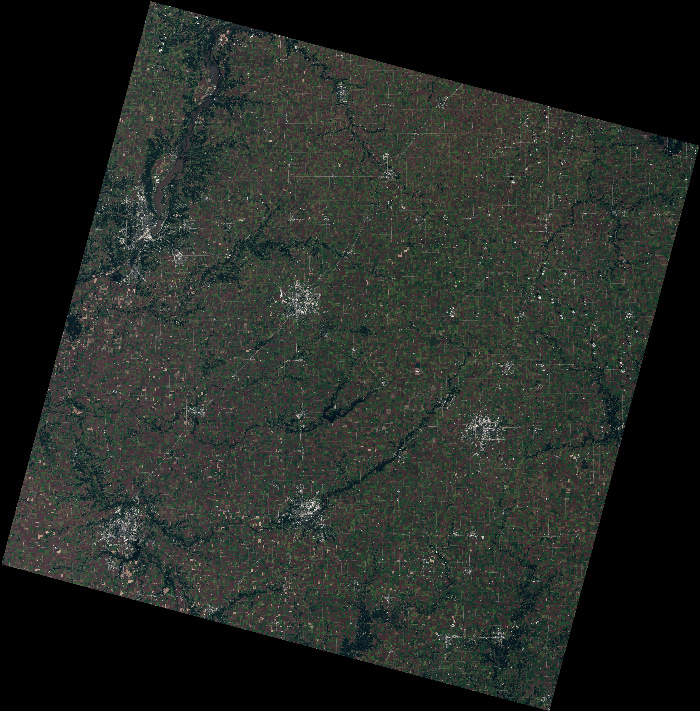
\includegraphics[width=\linewidth]{satellite}
\caption{Satellite RGB composite of central Illinois, capturing area of analysis}
\end{figure}

NDVI and NDWI were calculated separately and inserted into the feature vectors, given the values captured from each band given the following equations:

\begin{equation}
\begin{aligned}
NDVI &=  \frac{NIR - Red}{NIR + Red} \\ \\
NDWI_{Gao} &=  \frac{NIR - SWIR}{NIR + SWIR} \\ \\
NDWI_{McFeeters} &=  \frac{Green - NIR}{Green + NIR} \\ \\
\end{aligned}
\end{equation}

All models were built using default models provided by the scikit-learn python library.

\subsection{Crop Classification}
The method that yielded the best results for crop classification, using the provided features, turned out to be a random forrest classifier, using the \texttt{RandomForrestClassifier} method containing 10 estimators. Training and test subsets were then randomly allocated and divided from the overall dataset using the \texttt{train\_test\_split} method and passed to the K-Fold cross validator (consisting of 10 folds) for training and evaluation.

\subsection{Yield Estimation}
Support Vector Regression (SVR) was used to attempt to predict yields with the given multispectral measurements.  There was a preoccupation with attempting to find a 'best-fit' model that which produces a linear relationship between the features and yield, so a considerable amount of time was taken using trial end error to identify a model that would prove promising.

Unfortunately no regression technique emerged that yielded remotely usable results for the task at hand.  Further details are provided in the Evaluation section.

\begin{figure}[b]
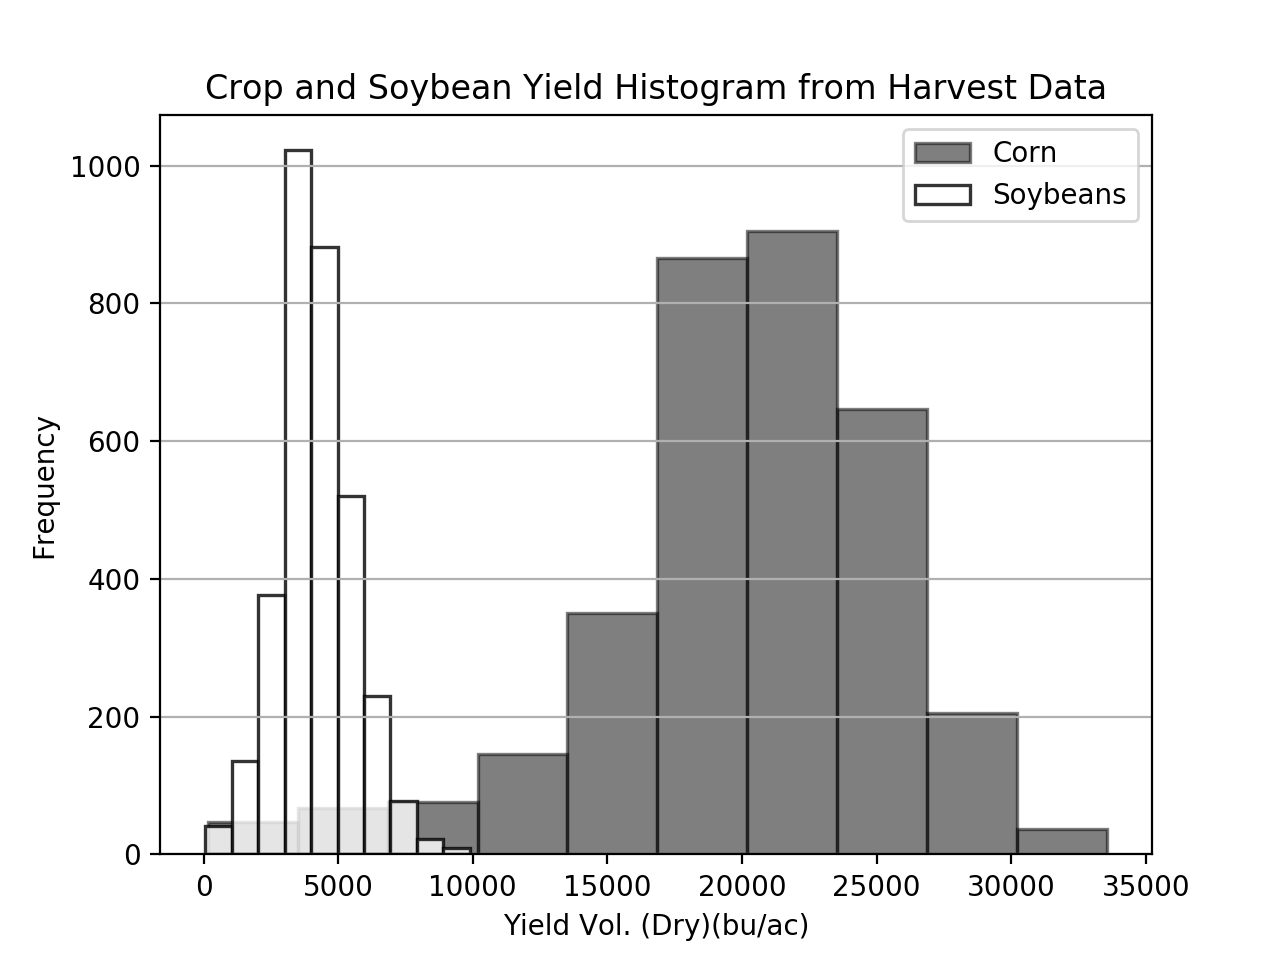
\includegraphics[width=\linewidth]{histogram}
\caption{Combined 2016-2017 harvest yield histogram}
\end{figure}

\section{Dataset}
\subsection{Contents and Features}
The availability of agricultural yield data was by far the largest limiting factor in the study.  Without an open source dataset, the effort focused on building and curating a dataset capable of supporting the task at hand -- an activity described in detail in the \textit{Data Curation} subsection.

The dataset is comprised of approximately 6,600 samples of 10 features consisting of multispectral band measurements obtained from Landsat 8 imagery (\textit{See Table \ref{record}}). For each record, two targets are provided with which to train -- yield and crop classification:

\begin{lstlisting}[language=Python]
In [2]: farm = load_data()

In [3]: farm.target_crop
Out[3]: array([1, 0, 0, ..., 0, 1, 0])

In [4]: farm.target_yield
Out[4]: array([  4033.,  20310.,  22225., ...,  26855.,   6188.,  29274.])

In [5]: farm.target_names
Out[5]: ['CORN', 'SOYBEANS']
\end{lstlisting}
\label{target}

\noindent
where the targets are one-to-one mapped to each record in order by index. \texttt{target\_crop} consisting of an array of labels whose values corresponds to the list of \texttt{target\_names}, and \texttt{target\_yield} consisting of yield measurements in bushel/acres.

\subsection{Data Curation}
The most difficult step was to obtain historical yield data from harvesting activities in the agriculture industry, which came in proprietary formats requiring third party software\footnote{ASF View by Chase IH was used to read and export harvest data collected from sensors onboard the farm equipment.} to parse and export into csv files. Harvest data described crop yield information accounting for 750 acres of farm land in central Illinois, covering two years of harvest activities.\footnote{2016-2017}

Based on harvest times, satellite imagery was identified and collected from the Landsat 8 satellite via the USGS website, where particular focus was placed on the Red, Green, Near Infrared (NIR), Shortwave Infrared (SWIR) and Thermal Infrared (TIRS) bands (\textit{See Table \ref{bands}}).

Using the Geospatial Data Abstraction Library (GDAL), lat/long measurements were correlated to pixels within the satellite images and the values within each band were extracted and concatenated into the feature set.  Additionally, for each record, the measured Red, Green, SWIR2 and NIR values were used to calculate the NDVI\cite{1974} and NDWI\cite{1}\cite{01431169608948714} as additional features.

The resultant dataset consisted of 10 features, with correlated crop types and yield sizes on a pixel by pixel level.  However, the number of measurements per pixel were not uniform, as the size and shape of the 750 acres of farmland being modeled were (obviously) not uniform 900m\textsuperscript{2} plots.  Using the number of samples per pixel, the dataset was further filtered to include only the records that were within three standard deviations from the median.

\begin{table}[t]
\caption{Record Example}
\label{record}
\begin{center}
\begin{tabular}{|c|c|}
\hline
\textbf{Feature} & \textbf{Value}\\
\hline
Green			&	8407		\\
\hline
NDVI			&	0.4495	\\
\hline
NDWI (Gao)		&	0.3661	\\
\hline
NDWI (McFeeters)	&	0.4008	\\
\hline
Near IR			&	19653	\\
\hline
Red				&	7464		\\
\hline
Shortwave IR 1		&	13473	\\
\hline
Shortwave IR 2		&	9119		\\
\hline
Thermal IR 		&	27287	\\
\hline
Thermal IR 2		&	24934	\\
\hline
\end{tabular}
\end{center}
\end{table}

\begin{table}[t]
\caption{Landsat 8 Band Designations\cite{rs61010232}}
\label{bands}
\begin{center}
\begin{tabular}{|c|c|c|c|}
\hline
\textbf{Band} & \textbf{Designation} & \textbf{Wavelength ($\mu$m)}& \textbf{Res (m)} \\
\hline
3 & Green & 0.0.533 - 0.590 & 30\\
\hline
4 & Red & 0.636 - 0.673 & 30\\
\hline
5 & Near Infrared (NIR) & 0.851 - 0.879 & 30\\
\hline
6 & Shortwave Infrared (SWIR) 1 & 1.566 - 1.651 & 30\\
\hline
7 & Shortwave Infrared (SWIR) 2 & 2.107 - 2.294 & 30\\
\hline
10 & Thermal Infrared (TIRS) 1 & 10.60 - 11.19 & 30$^{\mathrm{a}}$ \\
\hline
11 & Thermal Infrared (TIRS) 2 & 11.50 - 12.51 & 30$^{\mathrm{a}}$ \\
\hline
\multicolumn{4}{l}{$^{\mathrm{a}}$\textit{TIRS bands are acquired at 100 meter resolution, but are resampled to}}\\
\multicolumn{4}{l}{\textit{30m in delivered data product.}}
\end{tabular}
\label{band}
\end{center}
\end{table}


\section{Evaluation}
\subsection{Classification}
Random forrest classification performed at 89.7$\pm$0.2\% accuracy.\\

\subsection{Yield Estimation}
Methods consisted of permutations of performing standardization and principal component analysis (PCA) prior to being fed into linear regression models. SVR with radius bias function (RBF), linear, and polynomial kernels were also tested which yielded 0.02 r2 scores. Optimization was attempted upon the hyperparameters, for \(0 <= C <= 5\) and \(0 <= \gamma <= 100\), with no considerable improvements.

\section{Conclusion}
The use of current features extracted from multispectral sources indicates the probability there is no hard relationship between the gathered data and the yield. While this seemingly reenforces past methods utilizing datasets with wider temporal spread and/or physical parameters, not all factors have been considered in the course of the analysis described in this paper.

More interestingly, the potential use for crop classification using random forests does appear to be promising and could use additional attention.

\shrug\

\section{Acknowledgements}
Sincere thanks are due to Brent Lage, Dr. Jeremy Meiners and Dr. Chad Meiners for making this paper possible, and to Dr. Dennis Ross and Jacob Lowey for the guidance and direction.

\bibliographystyle{IEEEtran}
\bibliography{citations}


\end{document}
